\section{Construcció de l'Antena}

La construcció de l'antena dipol considerada consta de dues parts: el desenvolupament del balun i la construcció del cap de l'antena.

Cal mencionar que per a realitzar la construcció de l'antena, el paràmetre més important considerat ha estat que fos el més "low cost" possible sense comprometre la funcionalitat. Així doncs els materials utilitzats han estat:

\begin{itemize}
\item Filferro de 1.5 mm de diàmetre
\item Cable coaxial RG-59 de 75 ohms
\item Connector IEC 
\item Regleta 
\item Tupper
\item Termocola
\end{itemize}
\begin{figure}[H]
\centering
\begin{subfigure}{.5\textwidth}
	\centering
	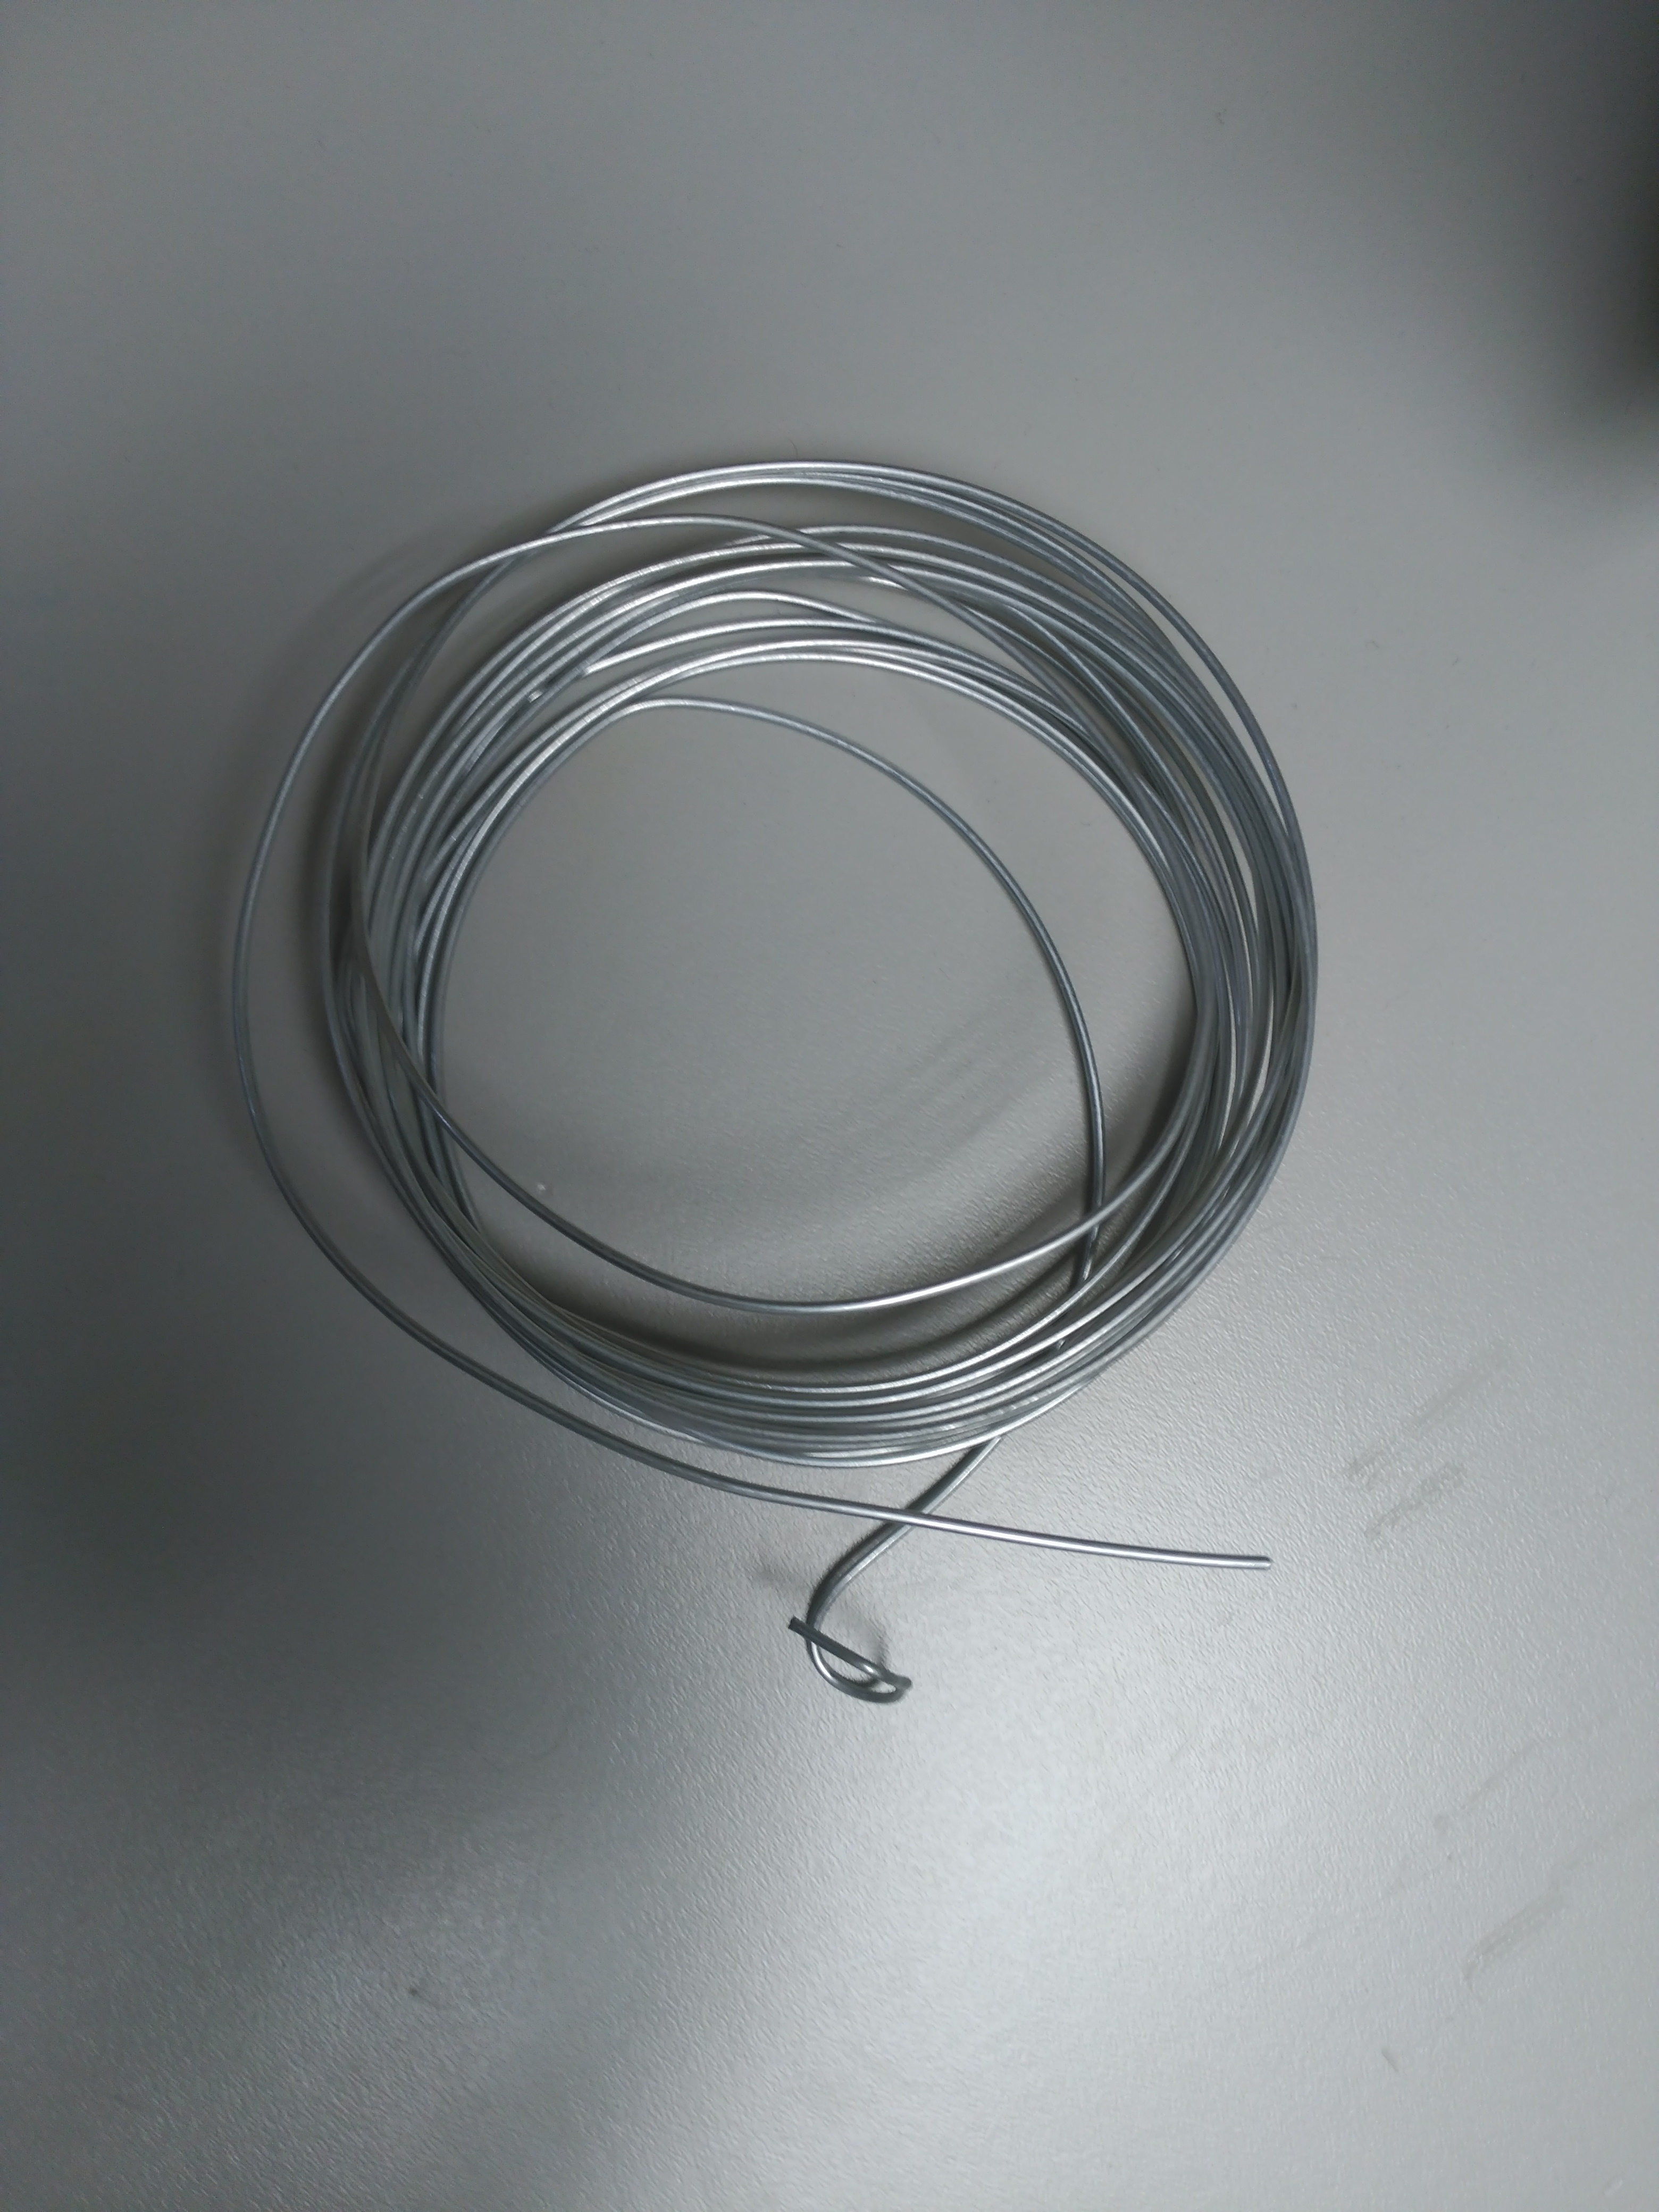
\includegraphics[width=0.9\textwidth]{./images/filferro.jpg}
	\caption{Filferro}
	\label{filferro}
\end{subfigure}%
\begin{subfigure}{.5\textwidth}
	\centering
	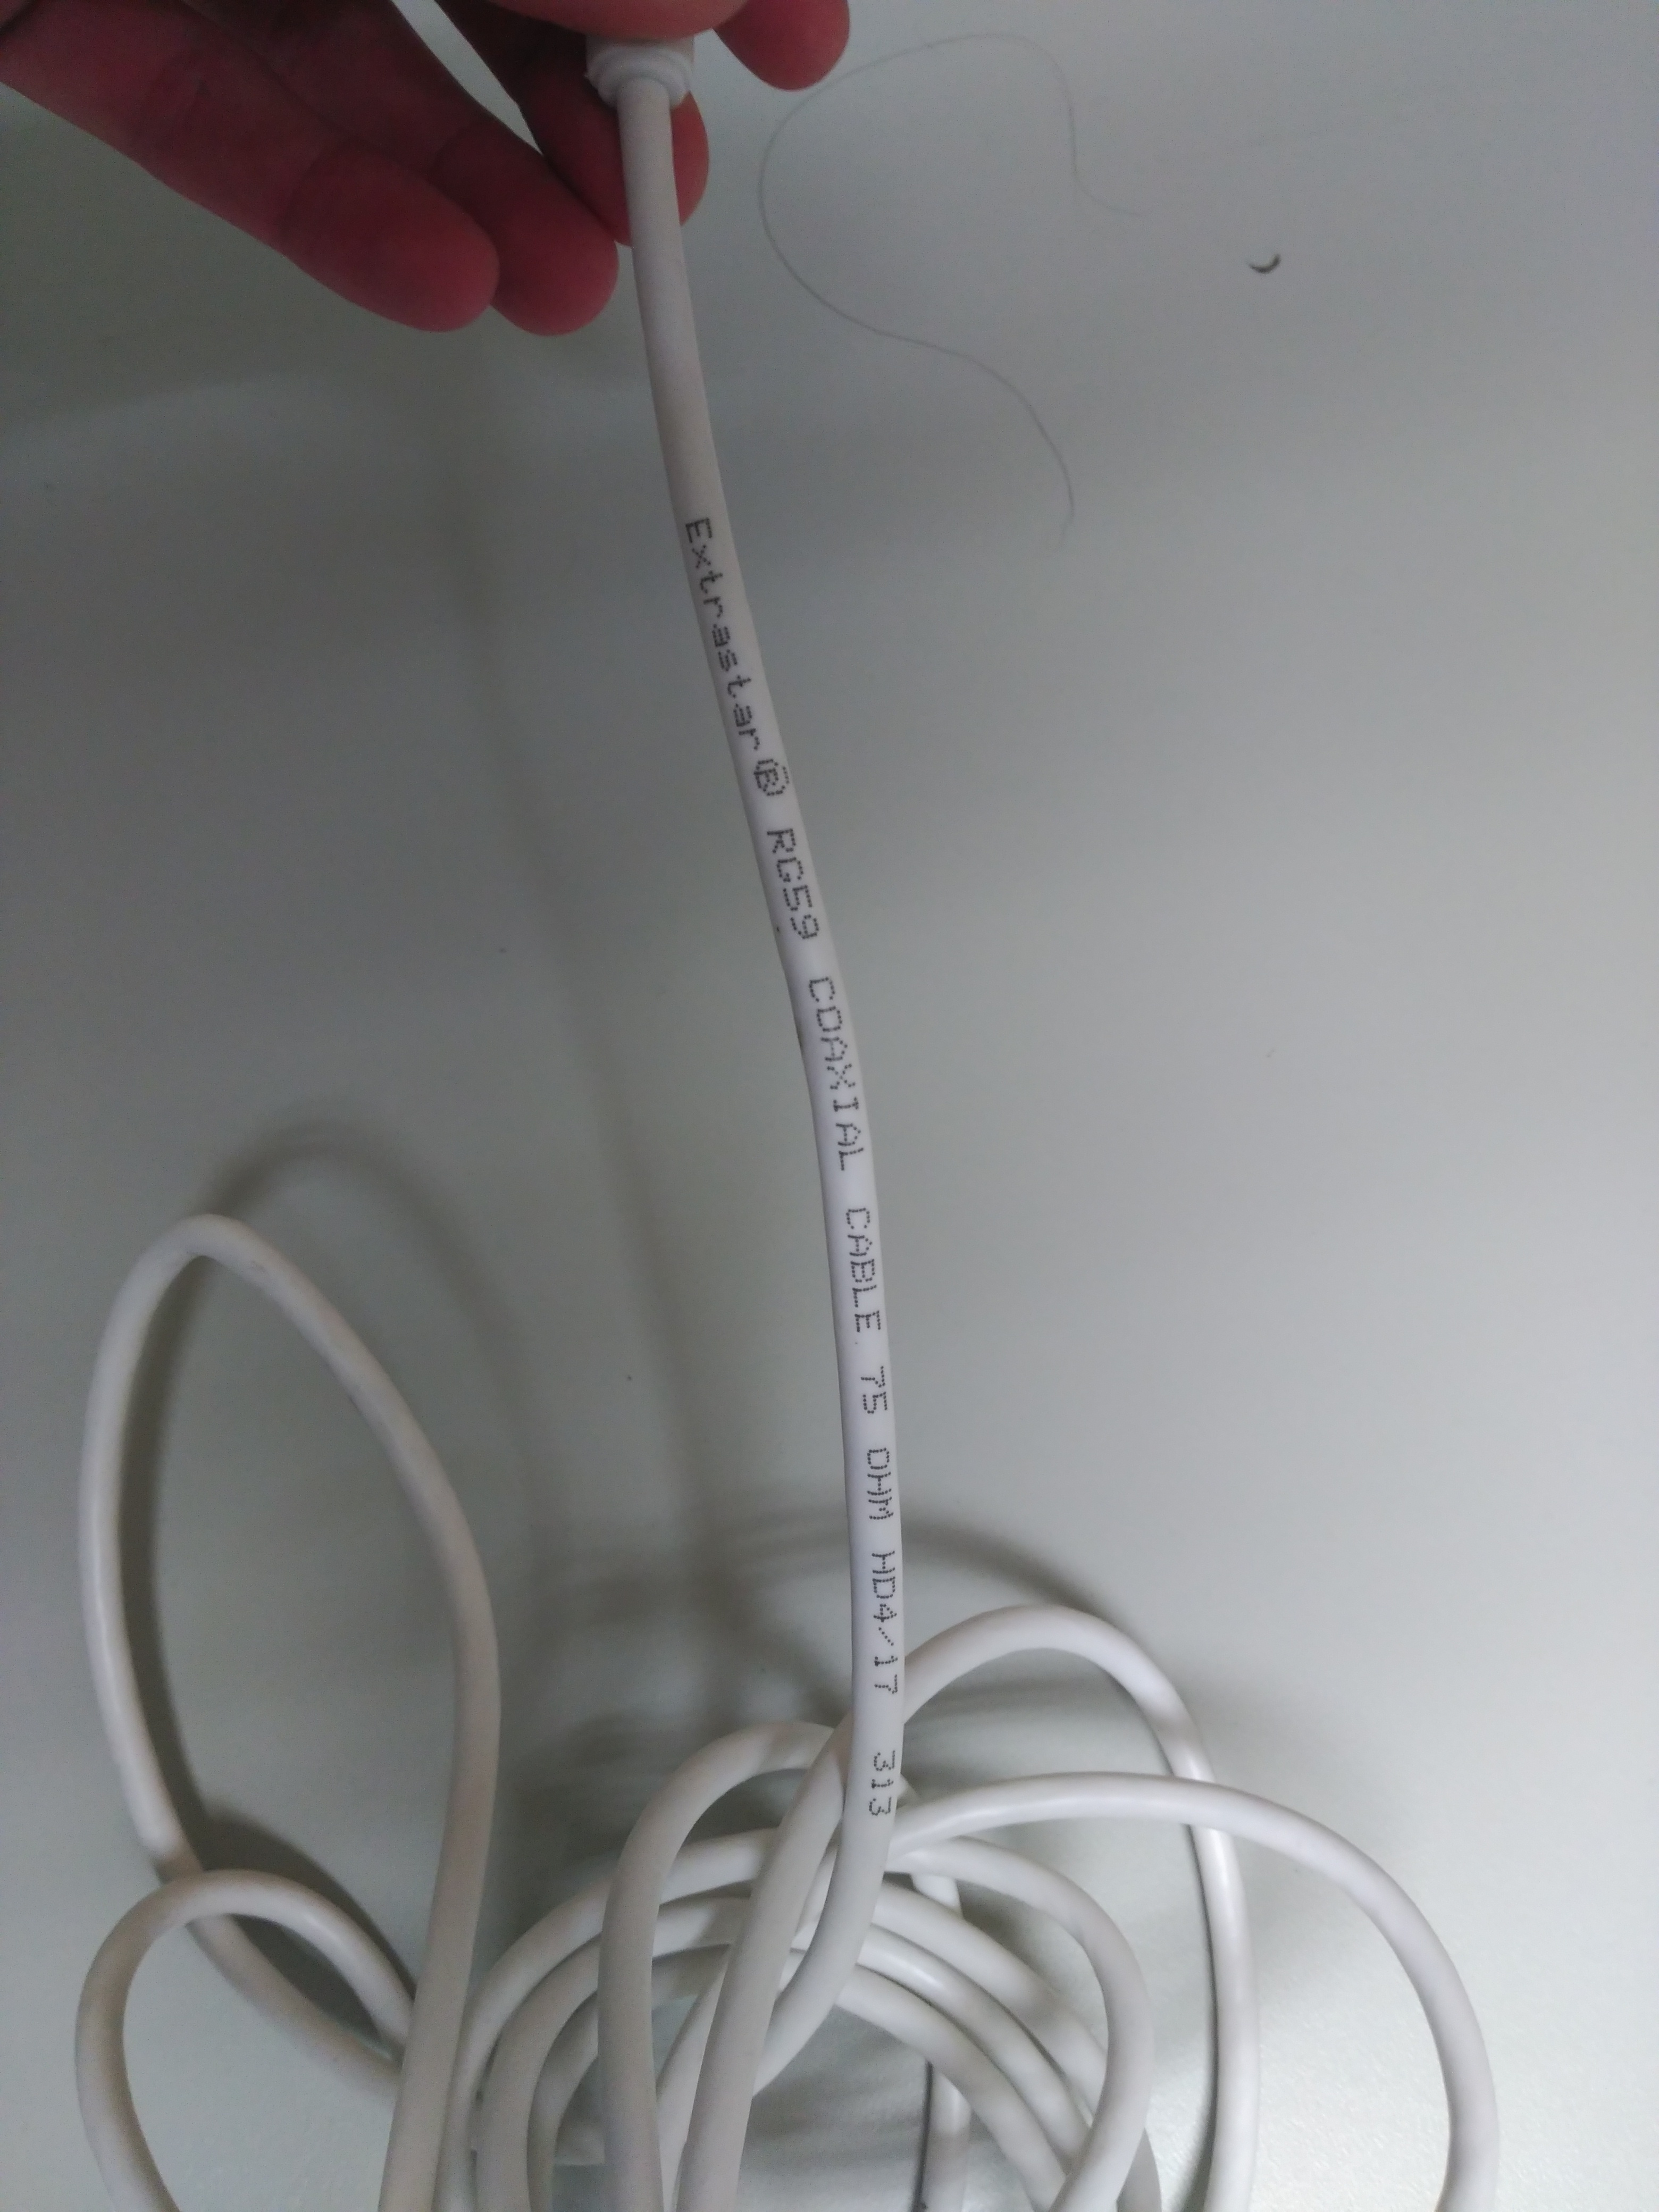
\includegraphics[width=0.9\textwidth]{./images/cable.jpg}
	\caption{Cable RG-59 de 75$\Omega$}
	\label{cable}
\end{subfigure}
\caption{Materials emprats}
\label{Materiales}
\end{figure}
\subsection{Balun}

Com s'ha escollit un dipol, aquest és un sistema balancejat mentre que el cable coaxial és un sistema no balancejat o \textit{"unbalanced"}. Per tant, es necessitarà una peça d'adapatació entre les dues xarxes. El \textit{balun}, com el seu nom indica, és una peça encarregada justament d'això. Aquesta era una complexitat afegida respecte al cas d'antena monopol doncs aquesta última no necessita un balun degut a que no és balancejada. 

Així doncs per fabricar el balun s'ha seguit el següent model extret de \cite{aznar2004antenas}:

\begin{figure}[H]
	\centering
	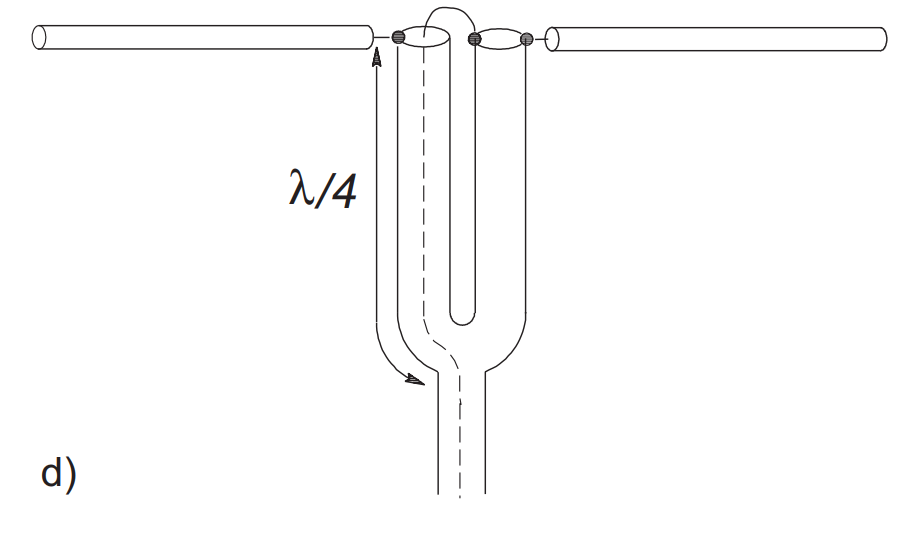
\includegraphics[width=0.6\textwidth]{./images/balun}
	\caption{Diagrama Balun $\lambda/4$}
	\label{balun}
\end{figure}

\begin{figure}[H]
\centering
\begin{subfigure}{.5\textwidth}
	\centering
	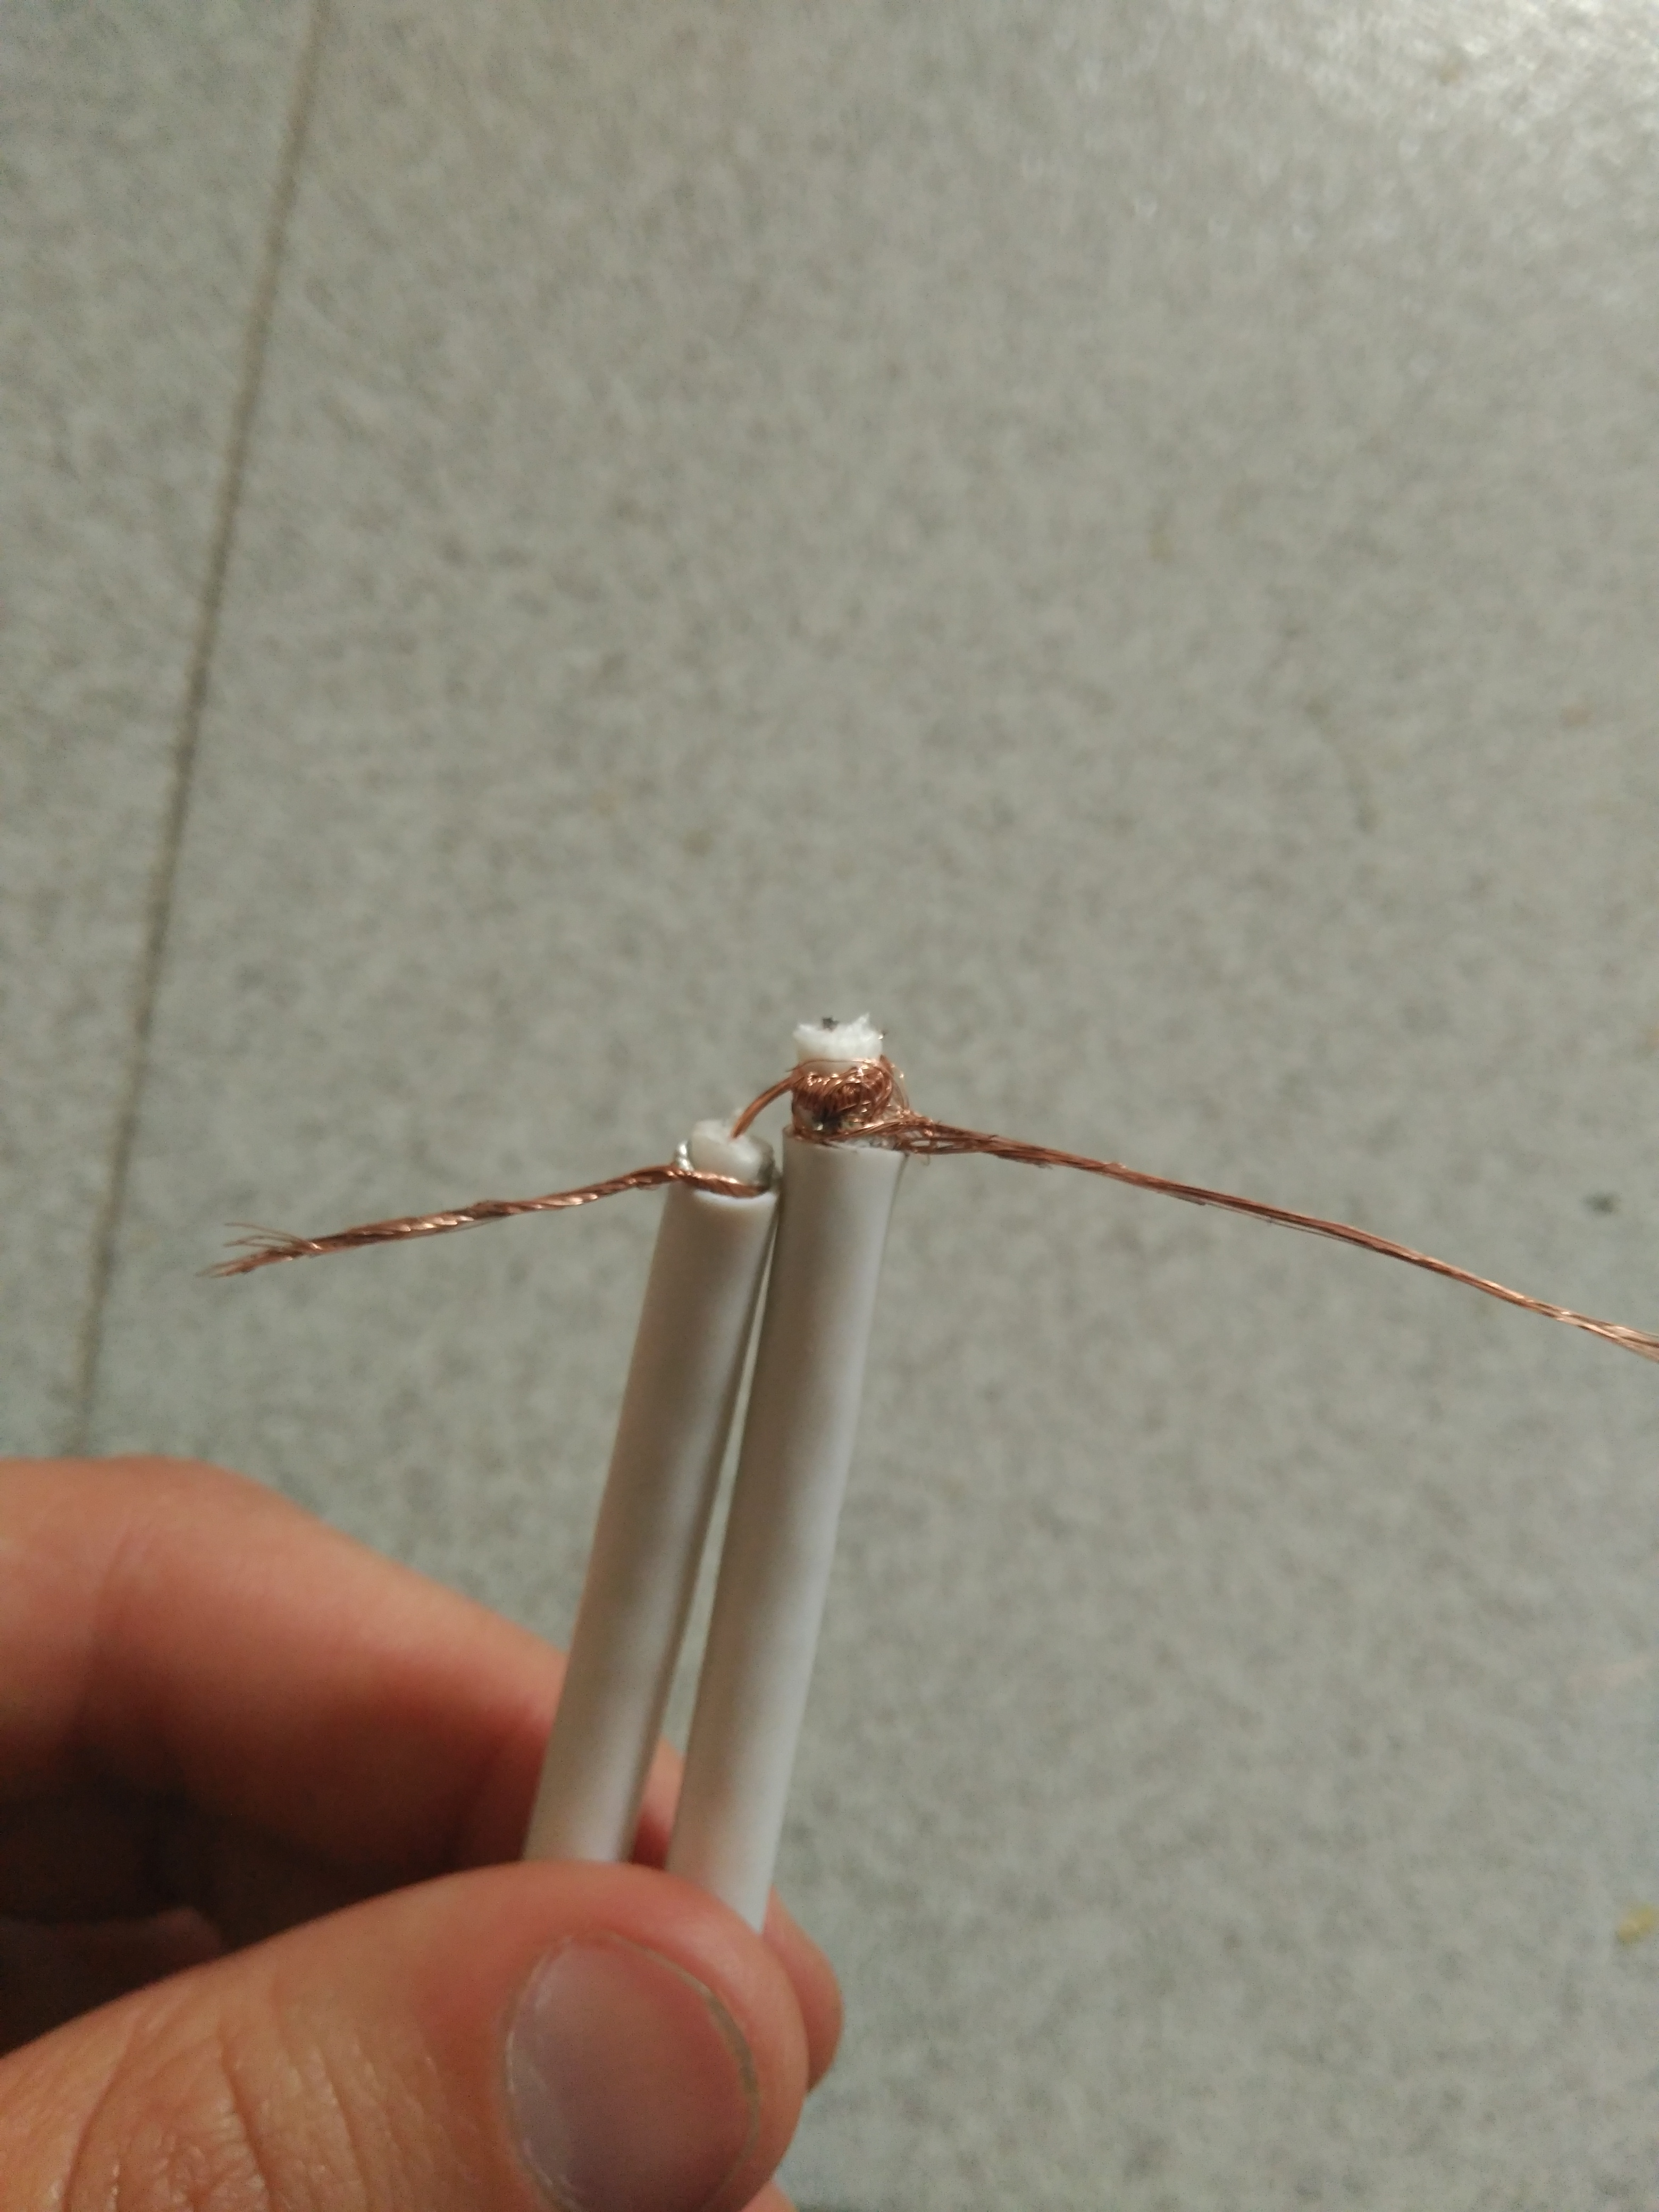
\includegraphics[width=0.9\textwidth]{./images/balun_pelat}
	\caption{Punta pelada}
	\label{balun1}
\end{subfigure}%
\begin{subfigure}{.5\textwidth}
	\centering
	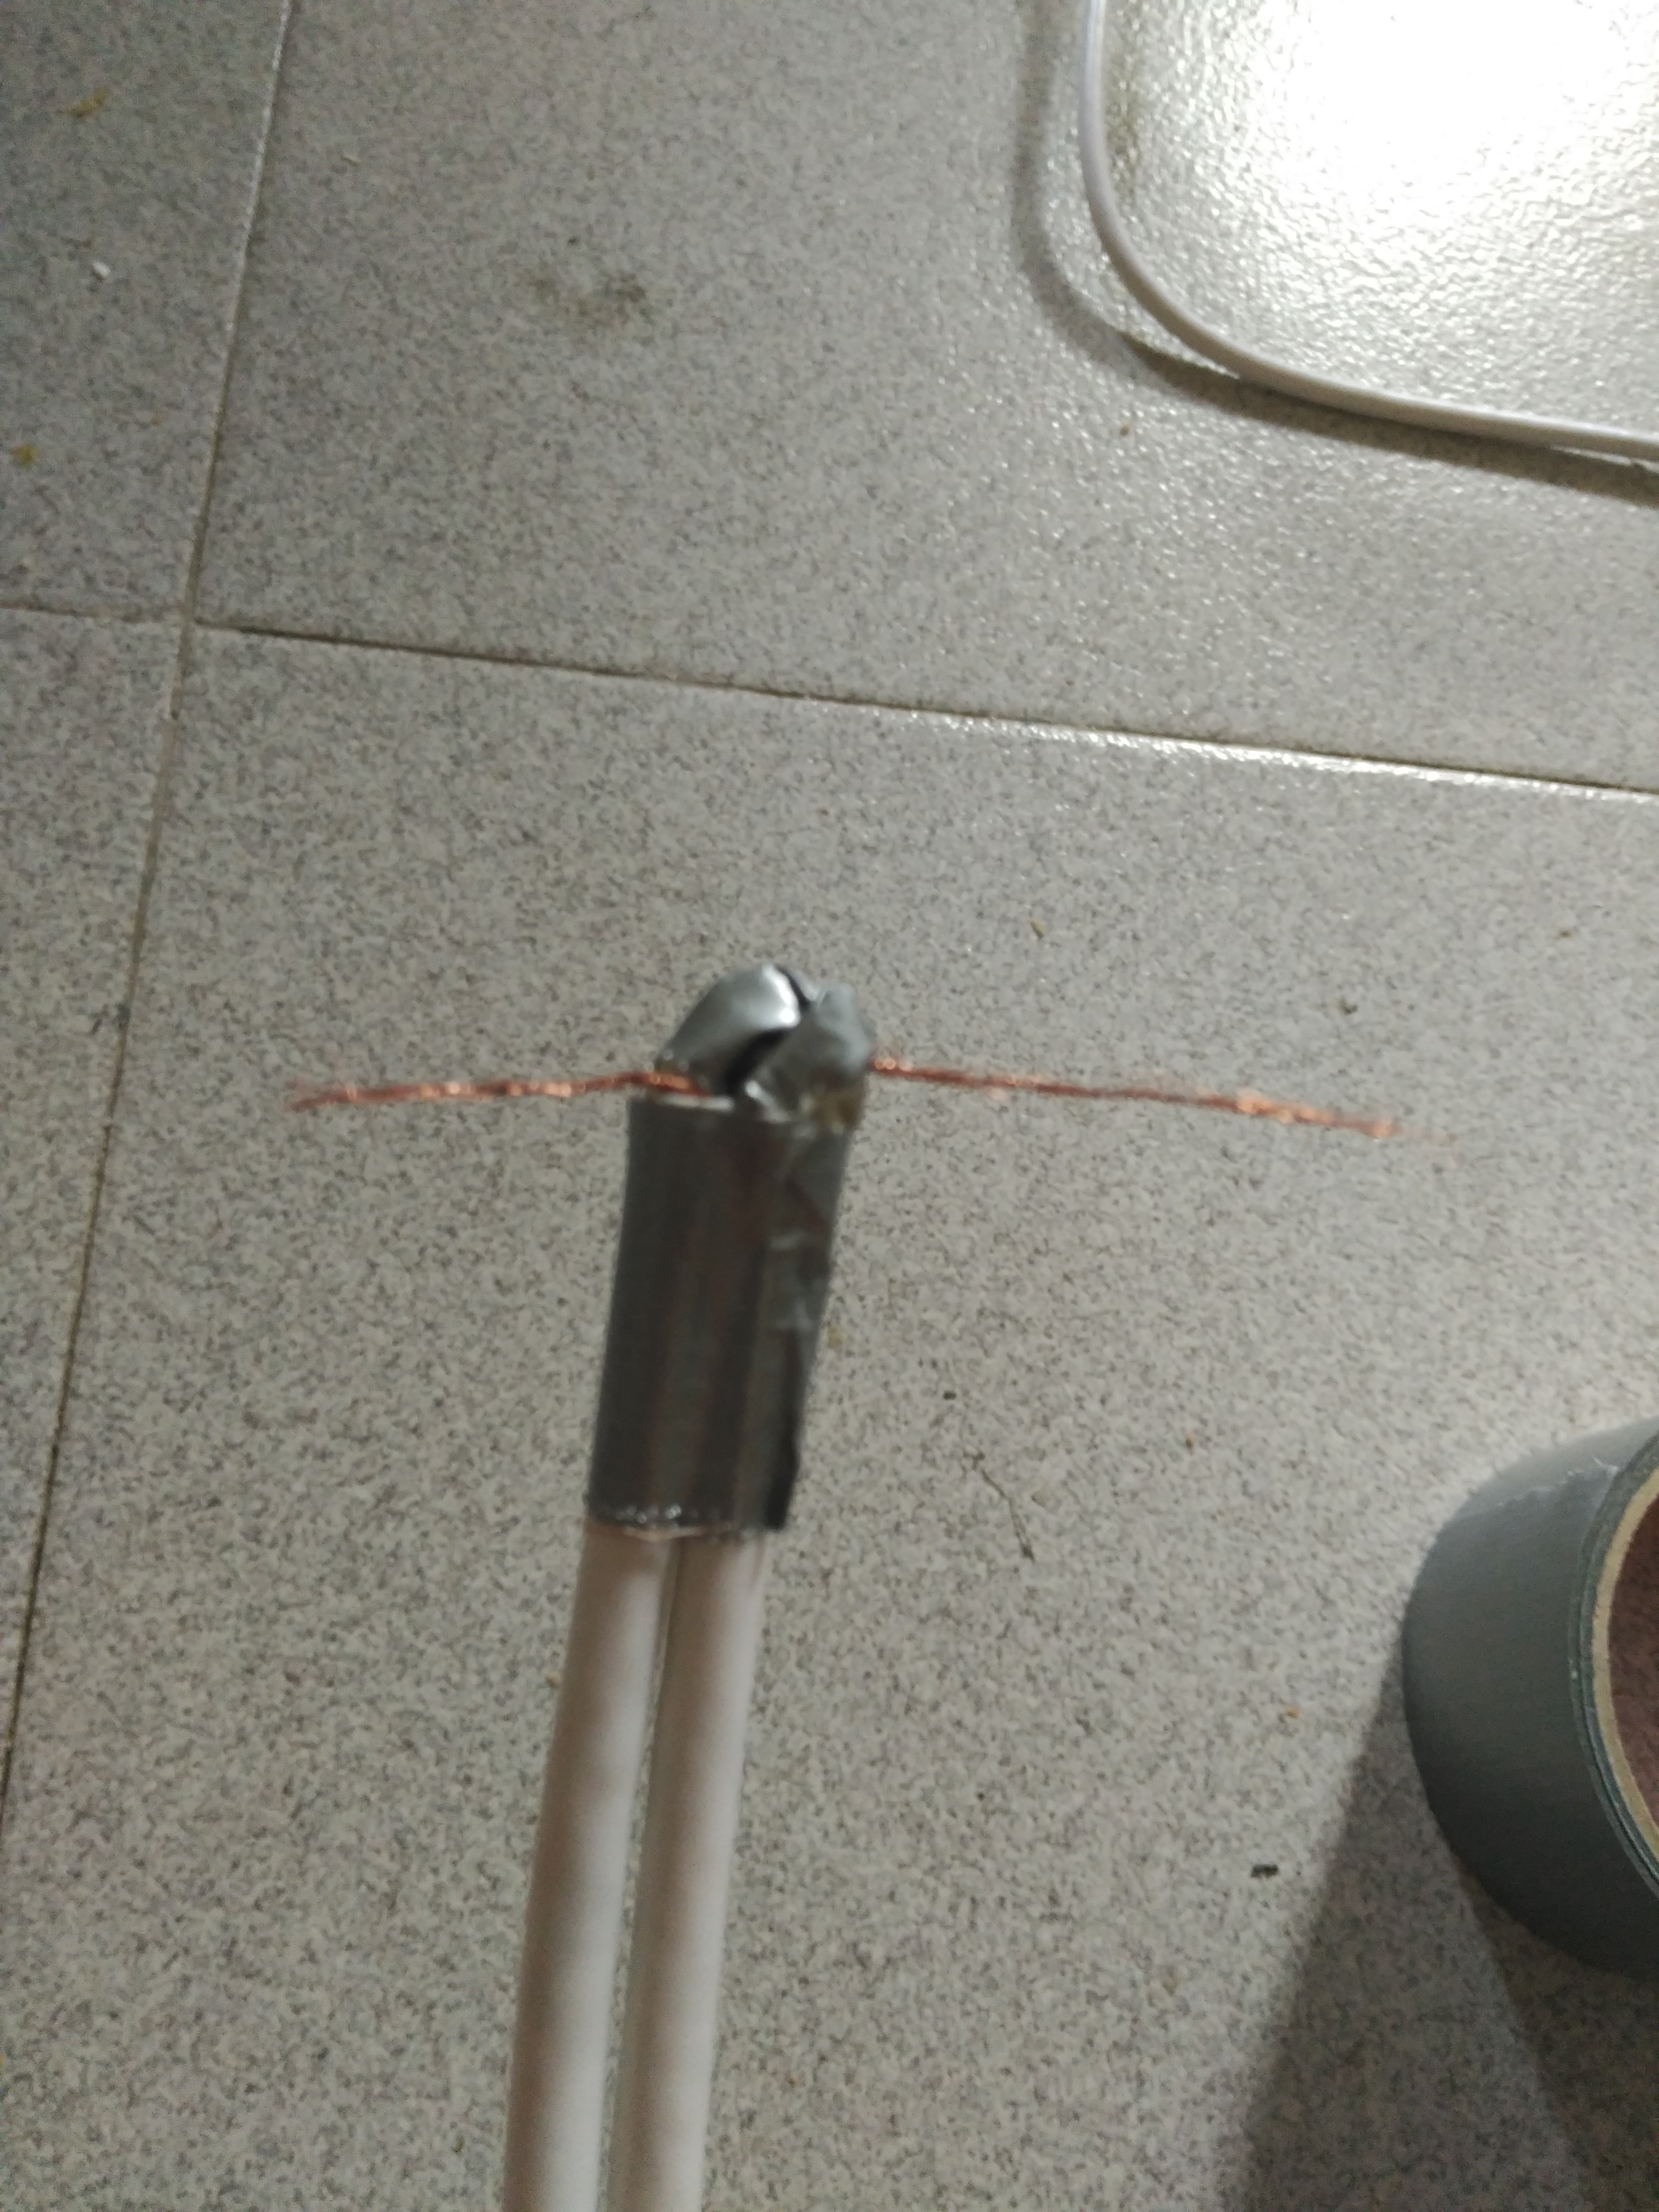
\includegraphics[width=0.9\textwidth]{./images/balun_aillat}
	\caption{Punta aïllada}
	\label{balun2}
\end{subfigure}
\caption{Balun $\lambda/4$ construït}
\label{baluncons}
\end{figure}

L'elecció s'ha basat en que aquesta configuració era la més senzilla que no modificava la impedància d'entrada. És recorda que el cable emprat és un RG-59 de 75$\Omega$ i que la impedància teòrica d'entrada de l'antena és de 73$\Omega$ degut a la longitud escollida. Per tant, el sistema està gairebé adaptat i no interessa que el balun modifiqui aquests valors.

S'observa el resultat del balun construït a la figura \ref{baluncons}.


\subsection{Cap de l'antena}

Per a la construcció del cap de l'antena s'ha utilitzat filferro de 1.5 mm de diàmetre així com una regleta per connectar els dos braços al cable d'alimentació.

A més, per tal de protegir les connexions (veure figura \ref{Conexions}), aquestes s'han dut a terme dins d'un \textit{tupper} i s'han aïllat posteriorment amb termocola. A més, per temes de seguretat, a les puntes del filferro s'ha posat termocola. %\ref{capAntena} 

\begin{figure}[H]
\centering
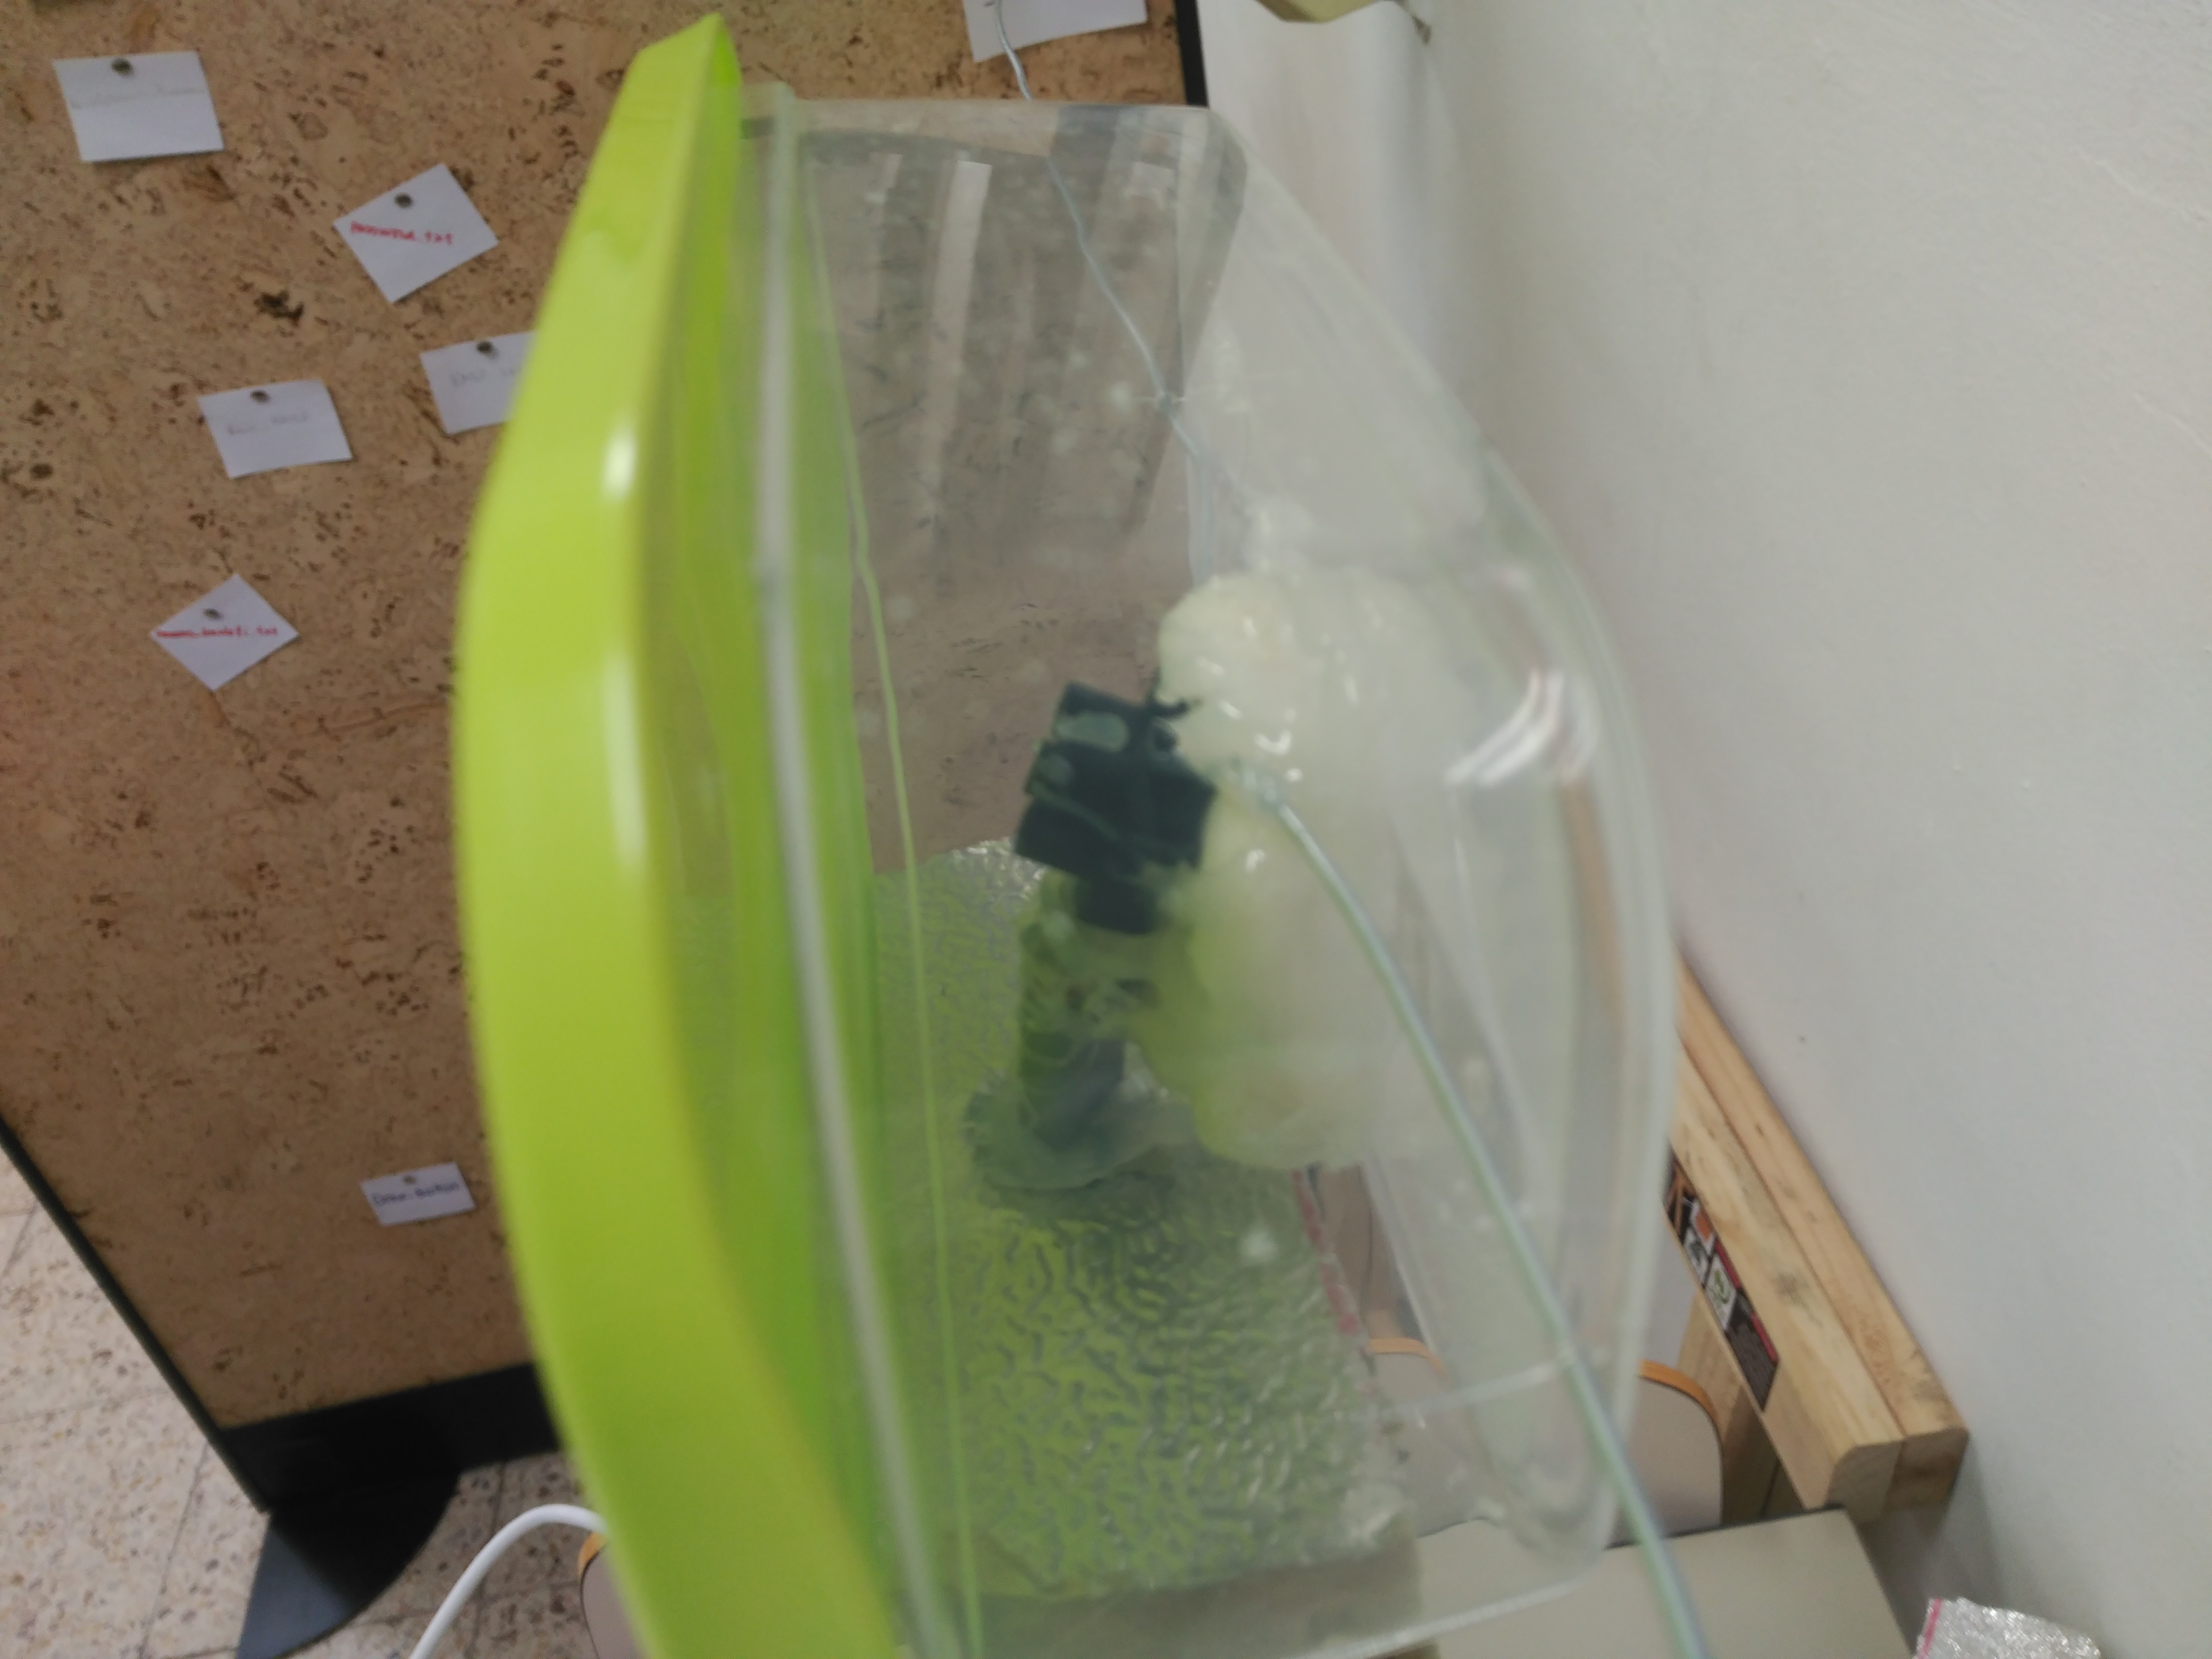
\includegraphics[width=0.5\textwidth]{./images/Conexions}
\caption{Conexions realitzades}
\label{Conexions}
\end{figure}

%((FALTA FOTO DE ANTENA DONDE SE VEAN LAS CONEXIONES))


\textbf{Antena Construida}

Finalment l'antena construida es la mostrada a la figura \ref{AntenaFinal}.

\begin{figure}[H]
\centering
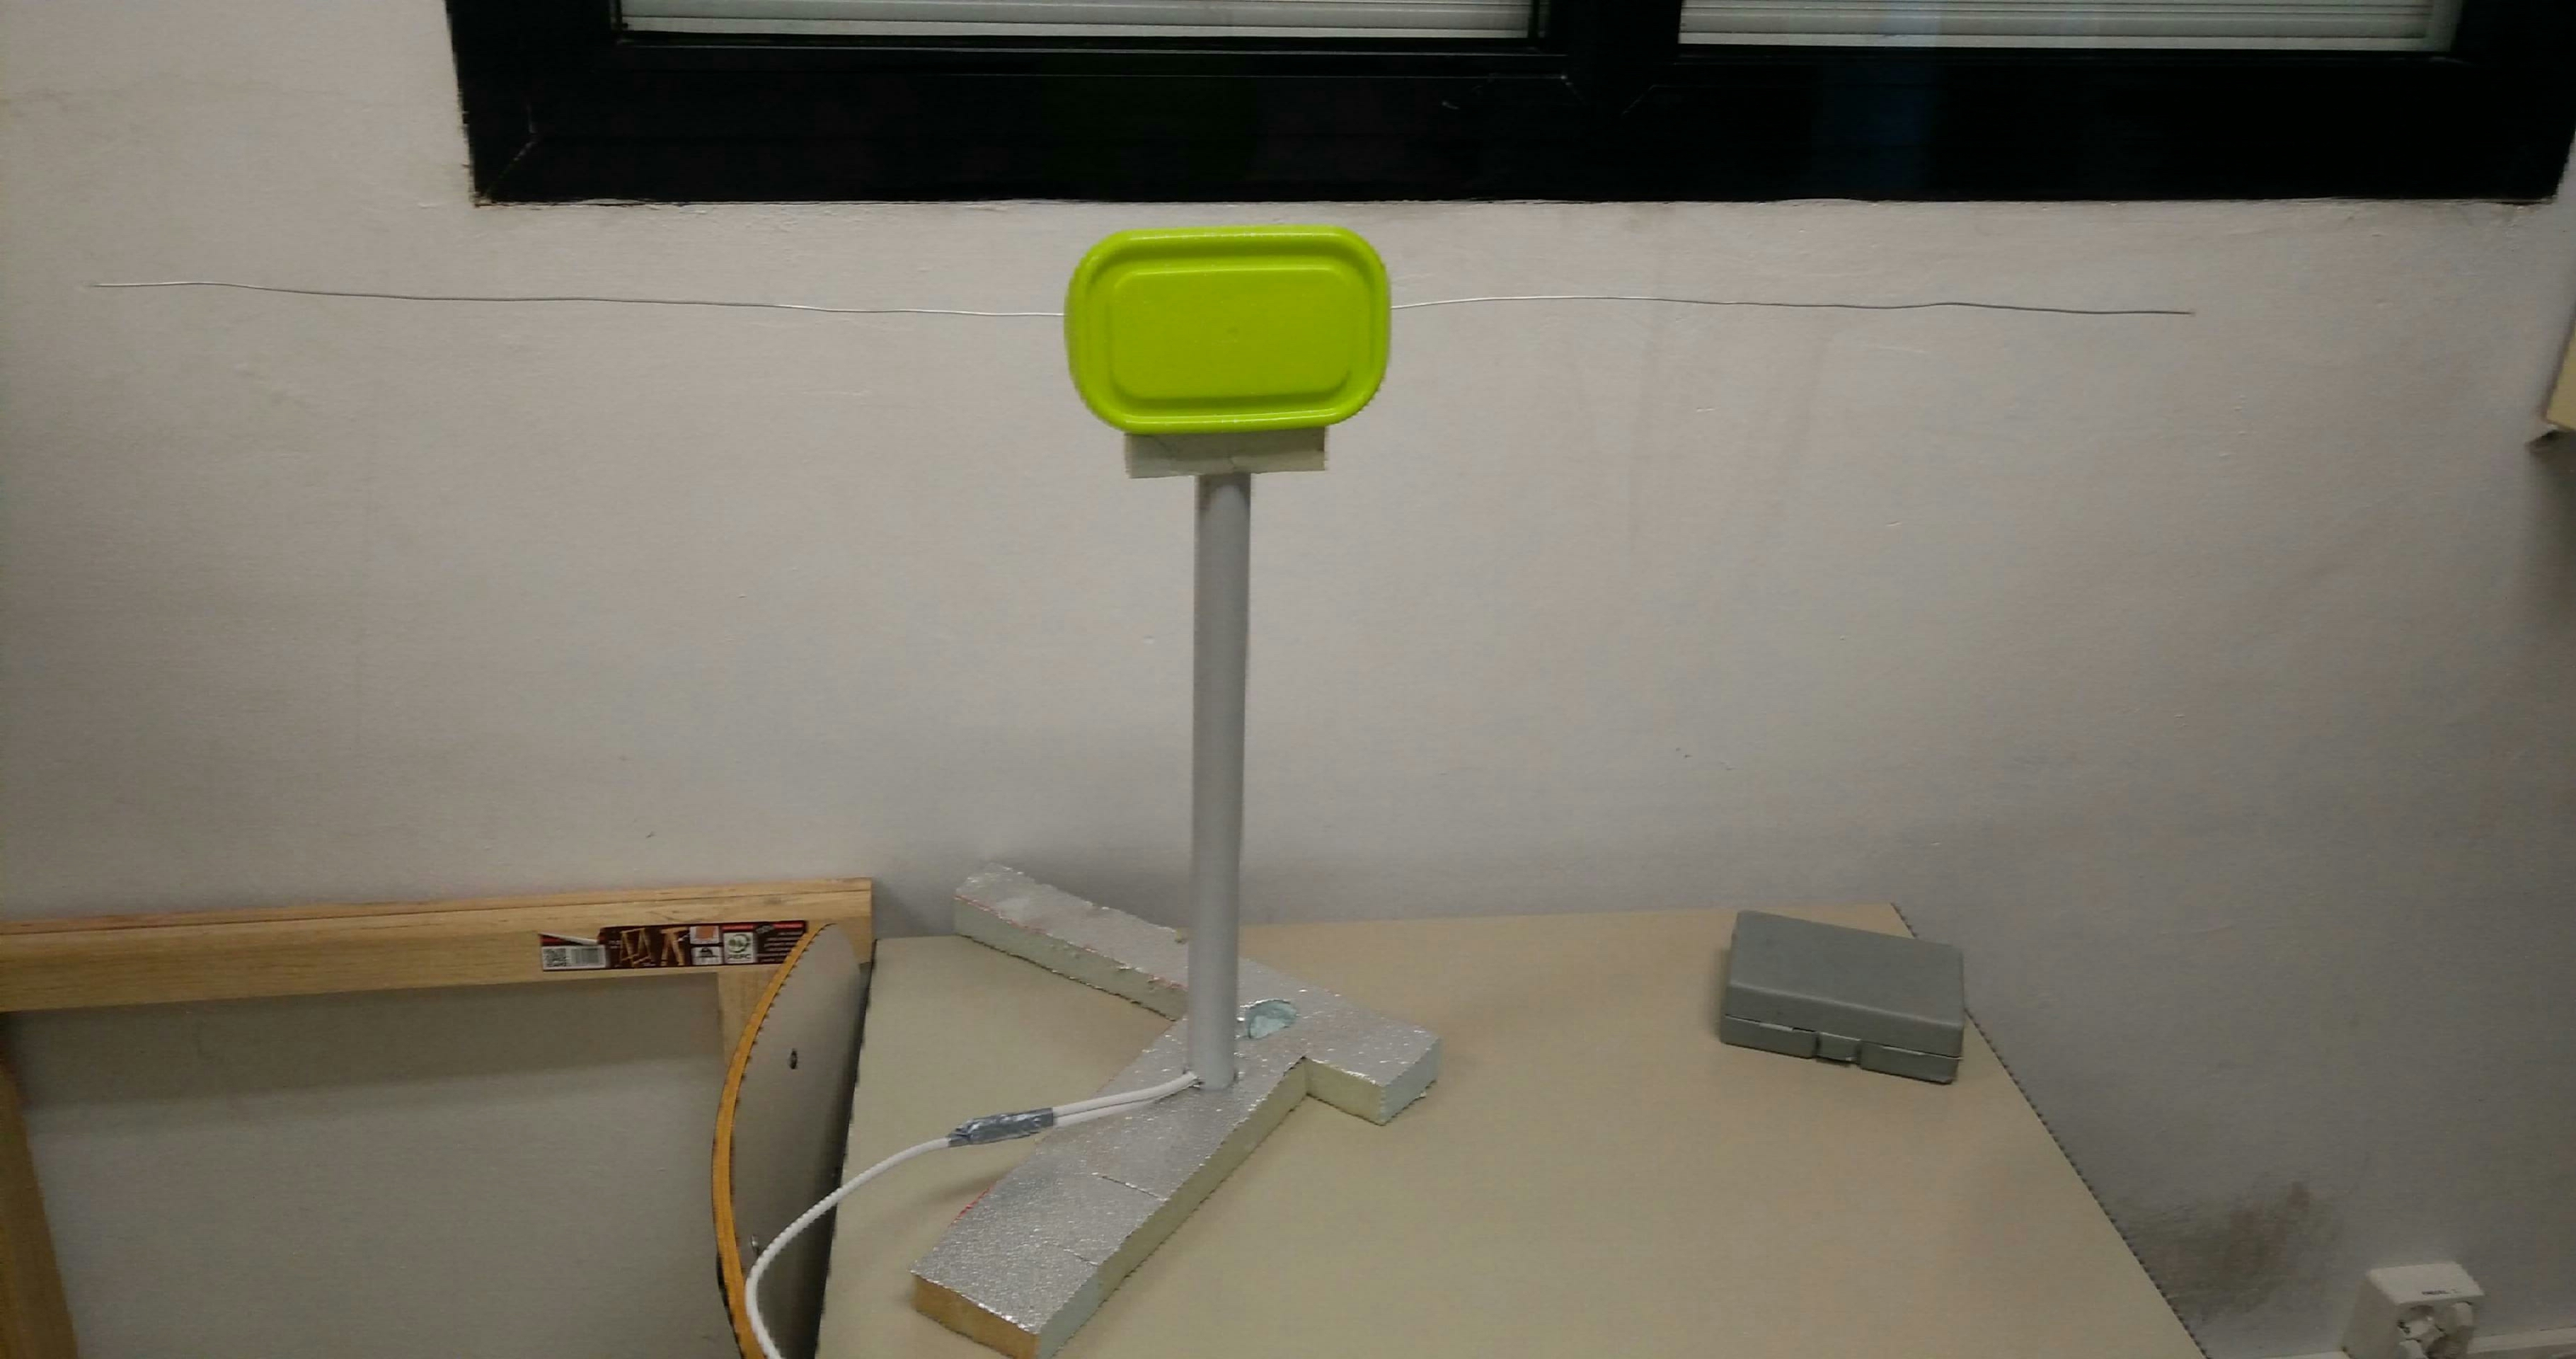
\includegraphics[width=0.8\textwidth]{./images/Antena_final}
\caption{Antena dipol construida}
\label{AntenaFinal}
\end{figure}